\documentclass[11pt]{article}
\pagestyle{plain}
\usepackage{color}
\usepackage{setspace}
\usepackage{caption}
\usepackage{subcaption}
\usepackage{fancyvrb}
\usepackage{epsfig}
\usepackage{fullpage}
\usepackage[small,compact]{titlesec}
\usepackage{hyperref}
%\usepackage{times} 
\usepackage{wrapfig}
\usepackage{enumitem}
\setlist{nolistsep}
\setlength{\topmargin}{+0.0in}   %%%%%%%%% this is hacked (from +.0.1in) so that it looks right when converted.
\setlength{\oddsidemargin}{-0.0in}
\setlength{\evensidemargin}{-0.0in}
\setlength{\textheight}{9.0in}
\setlength{\textwidth}{6.5in}
%\setlength{\parindent}{10ex}
%\setlength{\parskip}{\baselineskip}
\setlength{\parskip}{5pt plus 1pt minus 0.5pt}
\setlength{\parindent}{0pt}%
\bibliographystyle{unsrtnat}
\newcommand{\apj}{ApJ}
\newcommand{\apss}{Astrophysics and Space Science}
\newcommand{\aj}{AJ}
\newcommand{\apjl}{ApJL}
\newcommand{\mnras}{MNRAS}
\newcommand{\apjs}{ApJS}
\newcommand{\pasp}{PASP}
\newcommand{\pasa}{PASA}
\newcommand{\araa}{ARA\&A}
\newcommand{\aap}{A\&A}
\newcommand{\aaps}{A\&AS}
\newcommand{\pasj}{PASJ}
\newcommand{\prd}{Phys. Rev. D}
\newcommand{\nat}{Nature}
\newcommand{\physrep}{Physics Reports}
\newcommand{\etal}{et al}
\newcommand{\grackle}{\texttt{Grackle}}
\newcommand{\yt}{\texttt{yt}}
\def\subsun{\mbox{$_{\odot}$}}
\def\lesssim{\mathrel{\hbox{\rlap{\hbox{%
 \lower4pt\hbox{$\sim$}}}\hbox{$<$}}}}
\def\gtrsim{\mathrel{\hbox{\rlap{\hbox{%
 \lower4pt\hbox{$\sim$}}}\hbox{$>$}}}}
%\RequirePackage{natbib}
\usepackage[numbers]{natbib}
%\usepackage{setspace}
\setlength{\bibsep}{0.0pt}

\newenvironment{itemize*}%
{\begin{itemize}%
  \setlength{\itemsep}{0pt}%
    \setlength{\parskip}{0pt}}%
{\end{itemize}}

\newenvironment{enumerate*}%
{\begin{enumerate}%
  \setlength{\itemsep}{0pt}%
    \setlength{\parskip}{0pt}}%
{\end{enumerate}}

\newenvironment{description*}%
{\begin{description}%
  \setlength{\itemsep}{0pt}%
    \setlength{\parskip}{0pt}}%
{\end{description}}

\begin{document}

\clearpage

\clearpage
\begin{center} 
%\bfseries{%
%%
%% ENTER TITLE OF PROPOSAL BELOW THIS LINE
{\large PROJECT DESCRIPTION}\\
%%
%%
%}
\end{center}
\begin{flushleft}
\section{The \grackle{} Chemistry and Cooling Library}

The formation and evolution of astrophysical structures, such as
galaxies and molecular clouds, are governed
by a combination of non-linear phenomena, most notably gravitation,
hydrodynamics, and the atomic-scale physics that determine the
efficiency with which a plasma expels energy via radiative and
chemical processes.  Within simulation codes, gravity and
hydrodynamics solvers are relatively low-maintenance components, in
that they very rarely require updates due to advances in our
understanding of their processes.  Scaling is the only barrier to
increased sophistication.
In contrast, solvers for chemical and radiative processes are
extremely high-maintenance components, as the field of study they
represent evolves rapidly and is multifaceted, with advances coming
from theoretical calculations \citep[e.g.,][]{2007MNRAS.377..705F,
  2007MNRAS.382..133W, 2008MNRAS.388.1627G, 2008ApJ...689.1105L,
  2012JChPh.137o4303L, 2014ApJ...790...10S, 2015MNRAS.453..810L,
  2016MNRAS.457.3732C, 2017MNRAS.466.2175C} and laboratory experiments
\citep[e.g.,][]{2010Sci...329...69K, 2010PhRvA..82d2708B,
  2011PhRvA..84e2709M, 2015JPhCS.635b2092R, 2015ApJS..219....6O,
  2016ApJ...816...31D, 2016ApJ...832...31V}.  As a result, there
has been considerable divergence in the methods employed for solving chemistry
and cooling within the astronomical community.  This hinders scientific
progress by making it difficult to directly compare results from
different simulations and by mandating that considerable effort
within each research group be devoted keeping methods up to date.  The
\grackle{} chemistry and cooling library was developed with the
explicit purpose of addressing these problems, and its growing popularity
is a testament to its value to the community.

Gas chemistry presents a unique set of challenges in terms of
both computation and software development.  First, the network of
reactions rapidly grows in complexity with the number of elements and
species of those elements (i.e., the various ionization states and
molecular forms) considered.  For example, the simplest case of a
primordial gas consisting of hydrogen, deuterium, and helium minimally
requires between 11 and 15 species and roughly 20 to 30 reactions
\citep{1997NewA....2..181A, 1998A&A...335..403G}.
Adding just carbon and oxygen increases the minimal network to 
roughly 15-30 species and more than 50 reactions
and potentially up to almost 500, depending on the desired level of
accuracy \citep{2005ApJ...626..627O, 2012MNRAS.421..116G}.  Increases in
computational power will continue to be easily consumed by adopting
even gradually more sophisticated chemical networks and optimization
will remain critical.  An even greater challenge is that the
knowledge base
informing these solvers is continually evolving.  The rate
coefficients for many important reactions are still highly uncertain
\citep{2008MNRAS.388.1627G, 2011ApJ...726...55T} with accepted values
changing with new results from experimentation
\citep{2010Sci...329...69K, 2015ApJS..219....6O, 2016ApJ...816...31D}.
Additionally, new models are frequently created to account for
phenomena that are difficult to resolve or simulate directly, such as
UV background models that mimic reionization
\citep[e.g.,][]{1996ApJ...461...20H, 2001cghr.confE..64H,
2012ApJ...746..125H, 2009ApJ...703.1416F}, atomic
\citep{2013MNRAS.430.2427R} and molecular \citep{1996ApJ...468..269D,
2012MNRAS.425L..51W} self-shielding from photo-ionizing/dissociating
radiation, and heavy element cooling tables for metal-enrichment from
multiple sources \citep[e.g.,][]{2009MNRAS.393...99W,
2013MNRAS.433.3005D}.

Thus, a chemistry and cooling solver
represents, at best, a snapshot of an ever-evolving body of
knowledge.  The functionality provided by chemistry and cooling solvers is
absolutely vital to simulations and models of a broad range of
astrophysical problems: galaxy formation \citep{2016ApJ...830L..13M,
2016MNRAS.462.3265D, 2017MNRAS.465.2540P, 2017MNRAS.466..105A,
2017MNRAS.tmp..110D}; disk galaxies \citep{2015MNRAS.449.2588P,
2015ApJ...814..131G}; dwarf galaxies \citep{2017arXiv170108779H}, 
star formation \citep{2016Natur.535..523F, 2017ApJ...835..137W};
black hole formation \citep{2016MNRAS.459.3217L, 2016MNRAS.459.4209A,
2016MNRAS.459.3377R, 2016MNRAS.461..111R}; supernovae remnants
\citep{2012ApJ...748...12S, 2016arXiv161008528B, 2017MNRAS.465.2471G};
the interstellar medium \citep{2015ApJ...814....4L,
2016arXiv161201786K}; the intergalactic medium
\citep{2011ApJ...731....6S, 2011MNRAS.413..190T, 2012MNRAS.420..829O};
and reionization \citep{2014ApJ...789L..32K, 2015ApJ...811....3S}.
The tradition throughout the astrophysical simulation community has
been to develop in-house solvers, geared to the specific design of
each code and baked directly into the source, making abstraction and
direct comparison between codes extremely difficult.

\begin{figure}[h]
\begin{center}
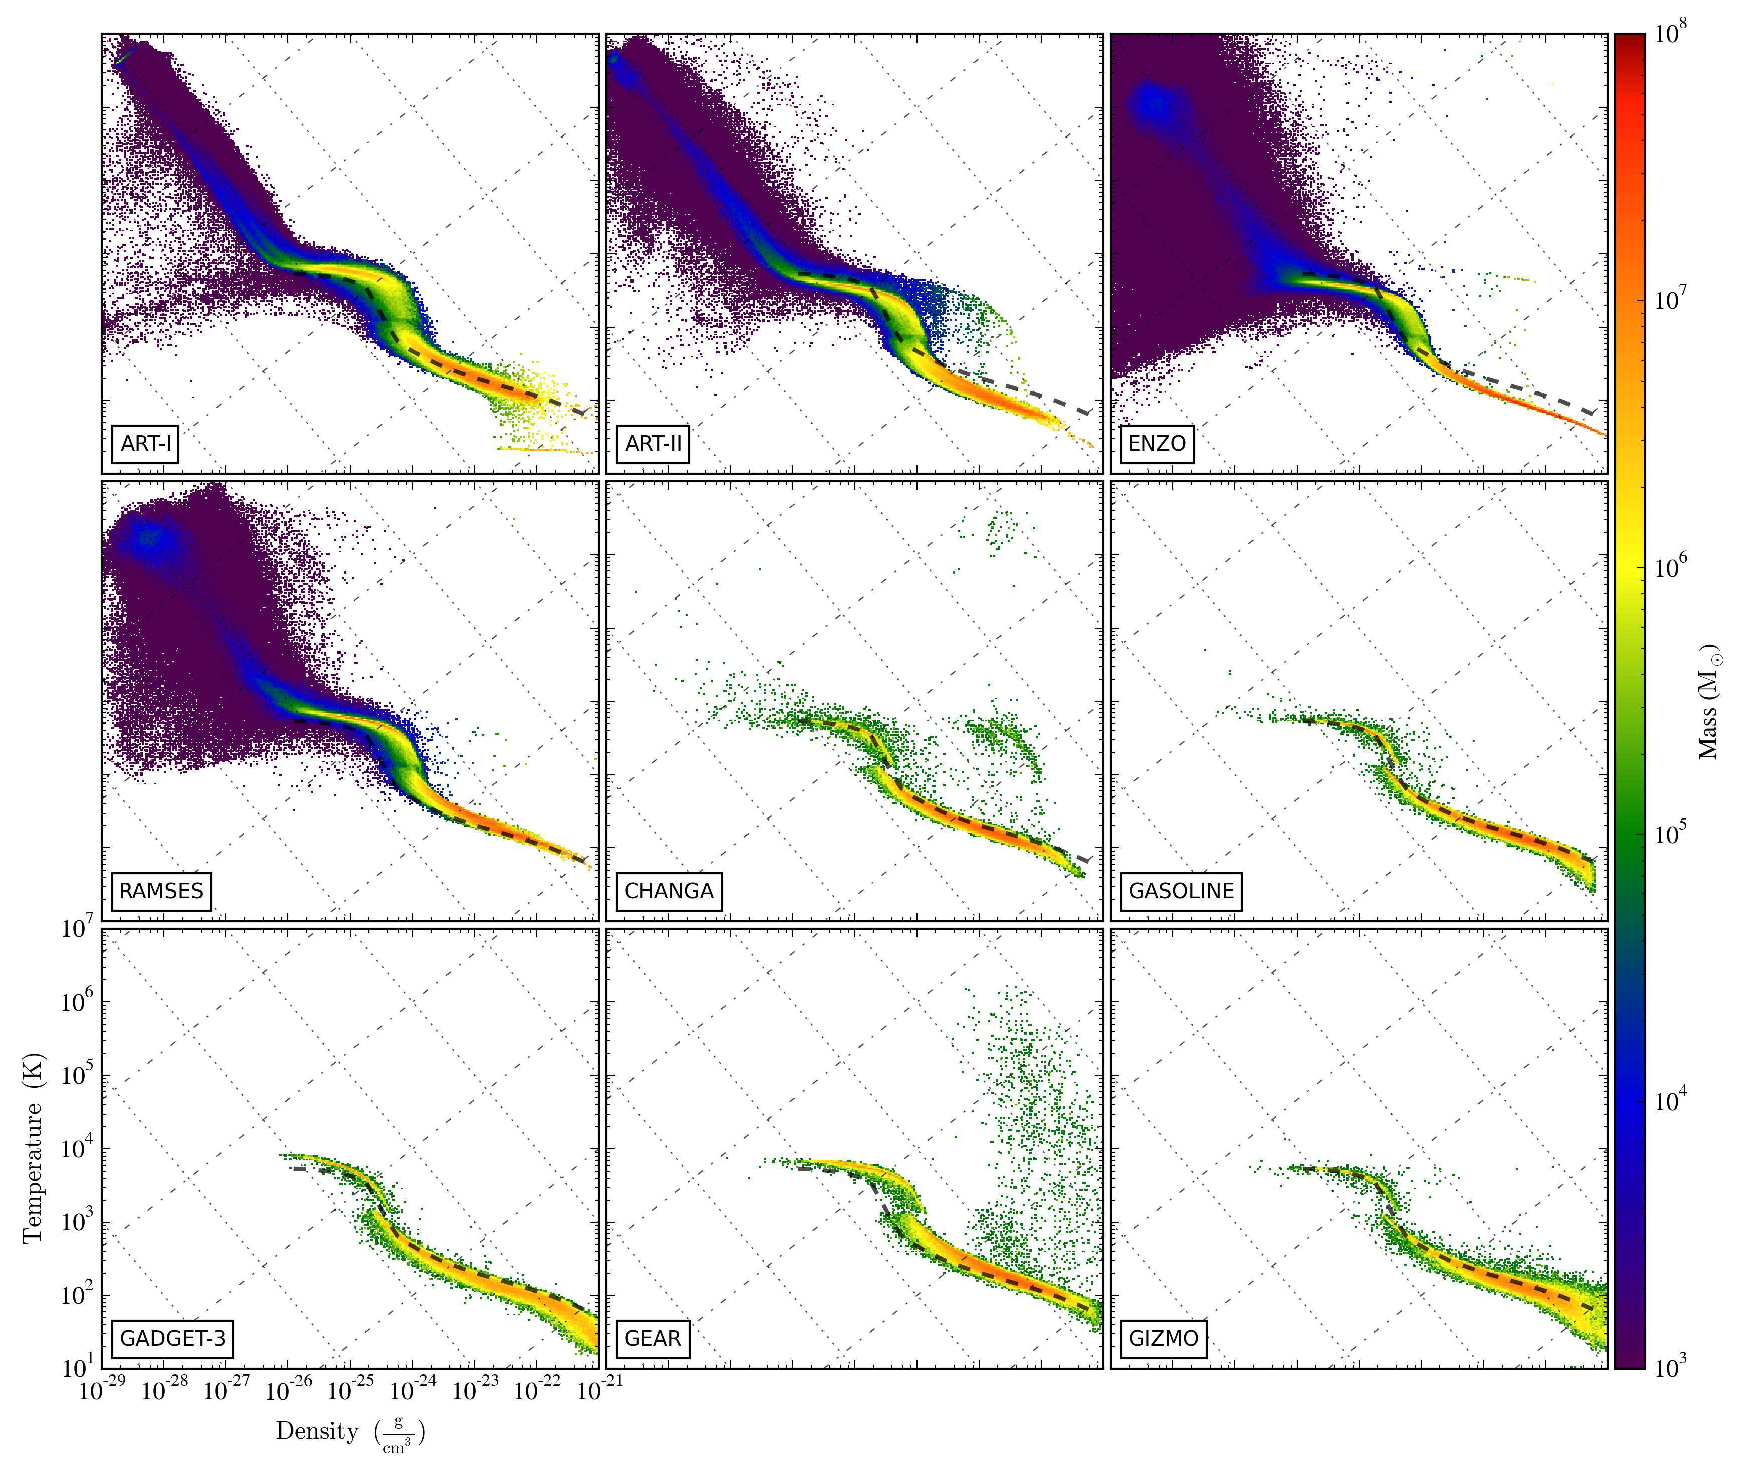
\includegraphics[width=0.92\textwidth]{figures/fig17.eps}
\caption{Figure 17 from \citet{2016ApJ...833..202K}, showing a
  comparison of nine simulation codes in the AGORA project, all using
  \grackle{}.  The panels show the probability distribution function
  in bins of density and temperature for the gas in isolated galaxy
  simulations.  Each simulation used an identical idealized setup,
  prescriptions for star formation and feedback, and radiative cooling
  provided by the \grackle{} library.}
\label{fig:AGORA}
\end{center}
\vspace*{-2\baselineskip}
\end{figure}

The \grackle{} project
\citep[][\url{https://grackle.readthedocs.io}]{2017MNRAS.466.2217S} is
an open-source library for computing the chemistry and radiative
cooling in astrophysical simulations and models.  The
\grackle{} library exposes functions necessary for computing the
thermal and chemical evolution of a collection of fluid elements carried by a
simulation.  These fluid elements can be either Eulerian (cells),
Lagrangian (particles), or a hybrid (e.g., moving mesh) with
application programming interfaces (APIs)
existing for codes written in C, C++, Fortran, and Python.  The
physical processes covered by the solver make it applicable to a broad
range of astrophysical topics, including star and galaxy formation, the
evolution of the intergalactic medium, and galaxy clusters.  Among
other metrics, the utility of \grackle{} can be demonstrated in two
important ways.  First, \grackle{} is a key component of the AGORA
\citep{2014ApJS..210...14K, 2016ApJ...833..202K} simulation comparison
project.  Comparing nine different simulation codes over multiple
galaxy formation problems, the AGORA project is the first
undertaking to include such a large fraction of the galaxy formation research
community.  An example of this cross-platform comparison enabled by
\grackle{} is shown in Figure \ref{fig:AGORA}.  Second, \grackle{} has
seen widespread adoption and use outside of participation in AGORA.
In total, \grackle{} has been adopted by at least 14 different
simulation codes:
AREPO, ART-I, ART-II, CHANGA, Cosmos++, Enzo, Gadget, GAMER, GASOLINE, Gear,
Gizmo, RAMSES, SPHS, and SWIFT
\citep{2010MNRAS.401..791S, 1999PhDT........25K, 2002ApJ...571..563K,
2008ApJ...672...19R, 2004NewA....9..137W, 2006MNRAS.373.1074S,
2003ApJS..147..177A, 2005ApJ...635..723A, 2014ApJS..211...19B,
2005MNRAS.364.1105S, 2010ApJS..186..457S, 2004NewA....9..137W,
2012A&A...538A..82R, 2012ASPC..453..141R, 2015MNRAS.450...53H,
2002A&A...385..337T, 2012MNRAS.422.3037R, 2013arXiv1309.3783G,
2016arXiv160602738S}.

\noindent
{\bf As an open-source project, \grackle{} plays two major roles:}
\begin{enumerate}
\item It provides access via a universal API to necessary functionality
that can be difficult for individual research groups to develop or
maintain on their own.  This increases overall productivity and
enables comparison and collaboration.
\item Second, by actively encouraging contribution though open source
  software best practices, it provides a means for dissemination of
  new methods and research results to the community.
\end{enumerate}
However, for \grackle{} to continue to be a useful resource, key
development projects must be undertaken to ensure that the code is
more inviting to new contributors and does not become a bottleneck
for effective utilization of next-generation computing facilities.
The purpose of this SSE is to support a series of specific
infrastructure and feature development tasks necessary for making
\grackle{} a self-sustaining community project by the end of the
three-year grant period.  The proposed tasks and their order of
completion have been designed to incrementally make the code more
attractive to external contribution and adoption by a wider audience.
The completion of each task will be marked by a major release of the
code.

\subsection{\grackle{} API}\label{sec:arch}

\grackle{} is a full-featured solver for gas chemistry and radiative
cooling with an API that is designed to minimize backward
compatibility issues and is straightforward to implement in simulation
codes written in C, C++, Fortran, and Python.  All functionality is
parallelized with OpenMP and can be used in hybrid MPI/OpenMP
frameworks.  To aid in semi-analytical
modeling and debugging of new features, it also includes a Python
interface with additional functionality.  Below, we detail the
features included and the functions provided to the user.

\grackle{} provides a non-equilibrium primordial chemistry solver for
atomic and molecular species of H, D, and He, including H$_{2}$
formation via three-body reactions \citep{2002Sci...295...93A,
2011ApJ...726...55T} and on dust-grain surfaces
\citep{1979ApJS...41..555H, 2000ApJ...534..809O, 2014ApJ...783...75M},
H$_{2}$ formation 
heating \citep{2009Sci...325..601T}, collision-induced H$_{2}$
emission \citep{2004MNRAS.348.1019R}, and HI
\citep{2013MNRAS.430.2427R} and H$_{2}$ \citep{2012MNRAS.425L..51W}
self-shielding.  The cooling from heavy elements up to atomic number
30 (Zn) is calculated by interpolating over tables of cooling and
heating rates created with the photo-ionization software,
\texttt{Cloudy} \citep{2013RMxAA..49..137F}.  These
tables are stored in HDF5 files included with the source.  For
increased speed at the expense of accuracy, the cooling from
primordial elements can also be computed using these tables.  In
addition to tables calculated assuming collisional ionization only
(i.e., no incident radiation), cooling tables have been created for two
different UV background models, those of \citet{2009ApJ...703.1416F}
and \citet{2012ApJ...746..125H}, in order to mimic the effects of
reionization.  For radiative transfer codes or simulation codes that
support radiation hydrodynamics, \grackle{} also allows the user to supply
photo-ionization and photo-heating rates for each computational
element.  Finally, arrays of arbitrary specific and volumetric heating
rates may be supplied to account for heating from stellar feedback
models and additional radiation sources.

The \grackle{} library exposes five primary functions useful to a
hydrodynamic simulation: 1) \texttt{solve\_chemistry} for iterating
the chemistry network and updating the species densities and internal
energy over a given time-step, and 2)
\texttt{calculate\_cooling\_time}, 3) \texttt{calculate\_pressure}, 4)
\texttt{calculate\_temperature}, and 5) \texttt{calculate\_gamma} for
computing the instantaneous cooling time, thermal pressure,
temperature, and ratio of specific heats, respectively.  Most of the
code's behavior is controlled by run-time parameters stored within a C
\texttt{struct} that is accessible from the main \grackle{} header
file.  The solver can be run with varying levels of sophistication,
including fully tabulated cooling, atomic chemistry only (6-species,
H, H$^{+}$, He, He$^{+}$, He$^{++}$, e$^{-}$), and additional tiers of
molecular chemistry (9-species adding H$_{2}$, H$_{2}^{+}$, H$^{-}$
and 12-species adding D, D$^{+}$, and HD).  Each of these, and other
optional features, requires a different number of fields to be carried
by the simulation code.  This functionality is exposed through
an API that has been designed to minimize the possibility of future
development breaking backward compatibility.

%% To maintain a single function signature,
%% regardless of chosen settings, field arrays are attached to pointers
%% within a C \texttt{struct} that is passed to the primary functions.
%% With this technique, new features requiring additional fields can be
%% added without altering function signatures, making the code
%% effectively backward compatible indefinitely.  This was an explicit
%% design decision made by the project to minimize future work required
%% by simulation codes using \grackle{}.

%\begin{wrapfigure}[20]{l}{0.50\textwidth}
%\vspace*{-2\baselineskip}
\begin{figure}
\begin{center}
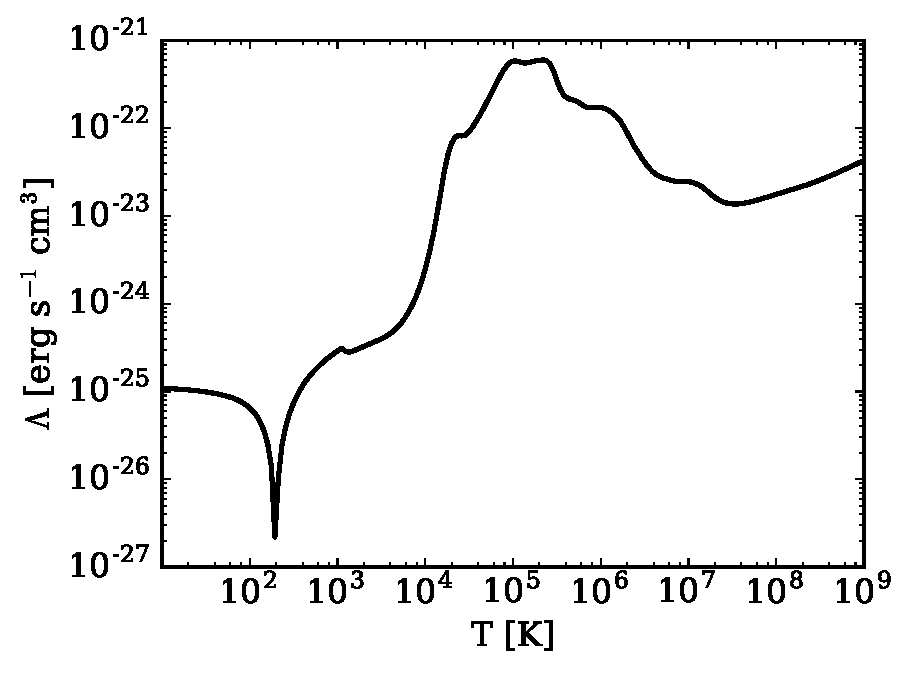
\includegraphics[width=0.48\textwidth]{figures/cooling_rate.pdf}
\caption{The cooling rate vs. temperature calculated by \grackle{}
  (using the \texttt{cooling\_rate.py} example script) for
  a gas with density of 10$^{-24}$ g/cm$^{-3}$ and solar metallicity,
  exposed to a radiation field described by the \citet{2012ApJ...746..125H} UV
  background model at redshift, z = 0.}
\label{fig:cooling-rate}
\end{center}
\vspace*{-1\baselineskip}
\end{figure}
%\end{wrapfigure}

\begin{figure}
\centering
\begin{subfigure}{.48\textwidth}
  \centering
  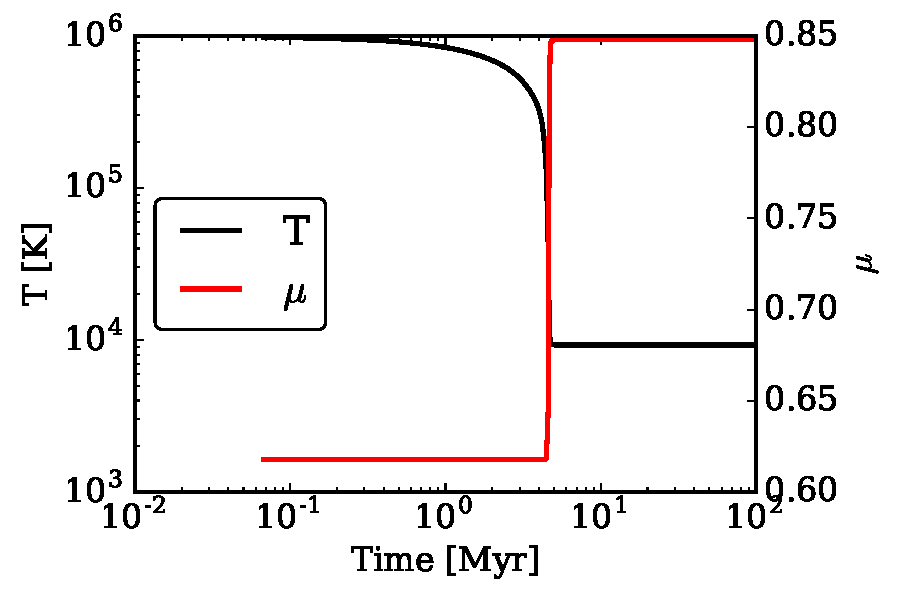
\includegraphics[width=0.98\textwidth]{figures/cooling_cell.pdf}
  \caption{Constant density model (\texttt{cooling\_cell.py}).}
  \label{fig:cooling-cell}
\end{subfigure}%
\begin{subfigure}{.48\textwidth}
  \centering
  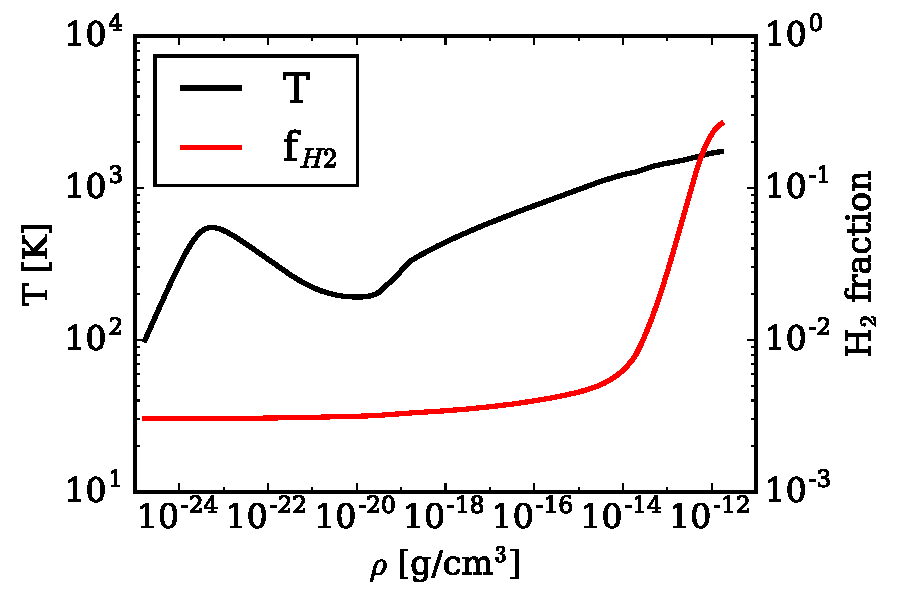
\includegraphics[width=0.98\textwidth]{figures/freefall.pdf}
  \caption{Free-fall collapse model (\texttt{freefall.py}).}
  \label{fig:freefall}
\end{subfigure}%
\caption{Example output from Python scripts included in the \grackle{}
  source using \texttt{pygrackle}'s helper functions for evolving
  fluid containers.}
\label{fig:evolve}
\vspace*{-1\baselineskip}
\end{figure}

\grackle{} has been designed to maximize scientific productivity on
high performance computing systems while maintaining an interface that
is immediately useful to people at many different levels of
experience.
All of the above functionality is easily accessible to codes written
in C, C++, and Fortran.  The \grackle{} source comes with compilable,
runnable examples in each of the above languages demonstrating all
available functions.  In addition, a Python module, \texttt{pygrackle},
is provided, exposing the main functionality as well as additional helper
functions useful in semi-analytic models, such as computing the
thermal evolution of a parcel of gas at constant density or undergoing
free-fall collapse.  Sample Python scripts are included in the source,
the running of which results in a figure of merit (shown in Figures
\ref{fig:cooling-rate} and \ref{fig:evolve}).

\subsection{\grackle{} Architecture}

\grackle{} is built upon widely used packages in the ecosystem of
scientific software.  As a library, the aim is to provide
functionality to the most commonly used programming languages in
scientific computing, namely, C, C++, Fortran, and Python.  The core
library is written in a combination of C and Fortran with the strategy
of using Fortran for the computationally expensive internal machinery
and C for user-facing functions and data storage.  The single
additional dependency is
HDF5\footnote{\url{https://www.hdfgroup.org/HDF5/}}, used for reading
cooling, heating,
and UV background rate data from input files.  HDF5 was chosen because
\grackle{}'s input files contain many data tables and the hierarchical
format makes them easily discoverable without prior knowledge of the
layout, allowing them to be easily reused by other codes.  The Python
interface makes use of a number of widely used Python packages, including
\texttt{NumPy}, \texttt{Cython}, and
\yt{}\footnote{\url{http://www.numpy.org/}, \url{http://cython.org/},
  and \url{http://yt-project.org/}, respectively} \citep[][an SI2-funded
project]{2011ApJS..192....9T}.  In
addition, the project infrastructure relies on the following packages:
Mercurial as the version control system; BitBucket.org to host the
main repository; Sphinx for building documentation; readthedocs.org to
host the latest build of the documentation; pytest for testing; and BitBucket
Pipelines for continuous integration testing.

\subsubsection{The Core Library}
\label{sec:core-library}

\noindent
{\bf Methodology}
Chemistry networks are challenging to solve because the time-scales of
reactions involved vary by many orders of magnitude.  These ``stiff''
networks are often solved using implicit methods, as they are able to
take longer time-steps than explicit methods, which are limited by the
shortest time-scale within the network.  However, a number of factors
can make an explicit scheme more attractive in certain situations,
particularly when the network is a component in a more complex physical
model governed by additional time-scales, as is the case here
\citep{2012JCoPh.231.5266G}.  Such factors include a higher
computational cost per solve with an implicit solver, steeper scaling
with the number of species, and the potential for hand-tuning of
explicit solvers for greater speed.  \grackle{} solves the primordial
chemistry network using an explicit method with a series of
optimizations shown by \citet{1997NewA....2..181A} to achieve
significant speedup with minimal cost to stability.  These
optimizations include replacing the fastest evolving species with
their thermal equilibrium values, tuning the order in which species
are updated, and switching between analytical and numerical time
derivatives when the system is close to equilibrium.  The time-steps
passed to \grackle{} from the simulation code are often much longer
than the relevant internal
time-scales.  To account for this, \grackle{} iterates in
``subcycles'' over time-steps limited by no more than 10\% of the
cooling time ($e/\dot{e}$) and chemical time-scales ($n/\dot{n}$) for
neutral H and for electrons.

\begin{figure}[h]
\centering
\begin{subfigure}{.54\textwidth}
  \centering
  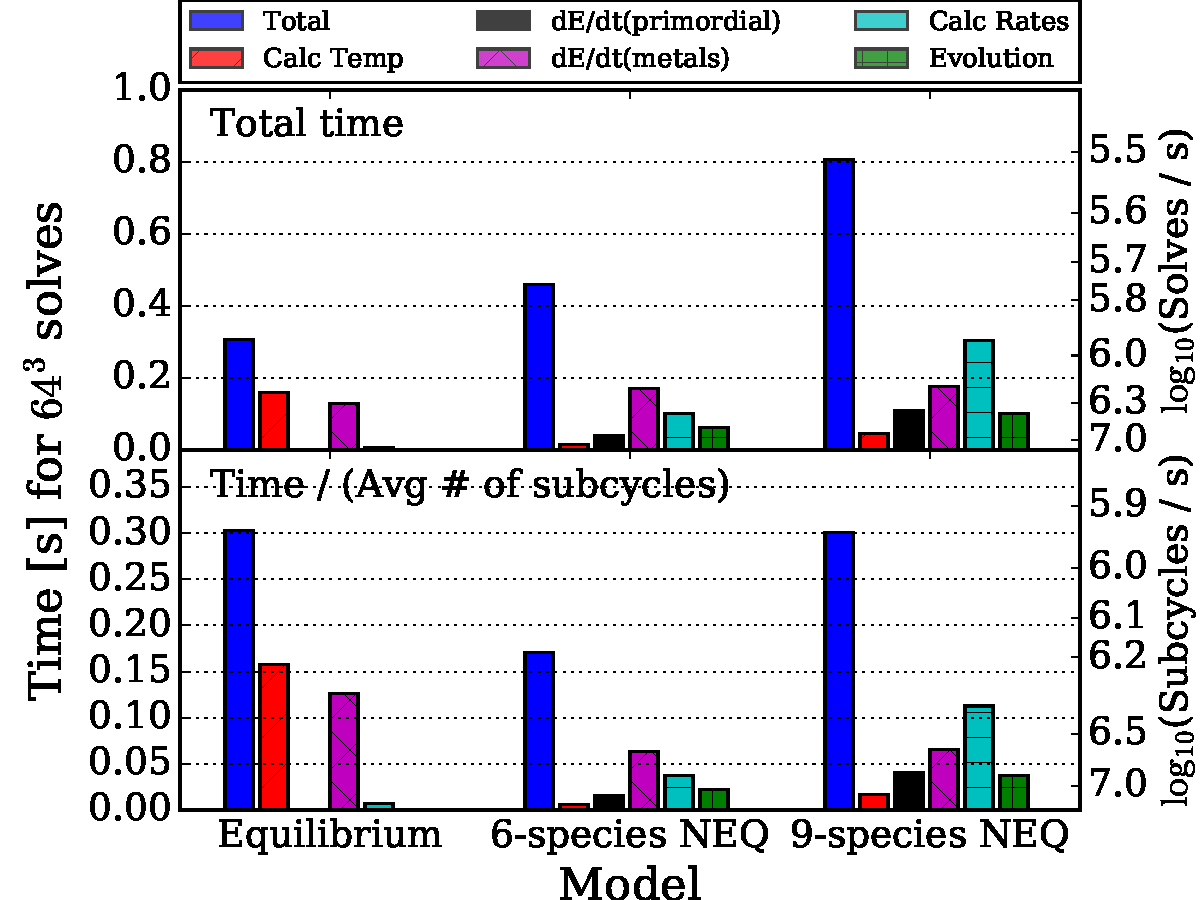
\includegraphics[width=0.98\textwidth]{figures/performance.pdf}
  \caption{Serial performance - Top: time
    to integrate a fluid container with 64$^{3}$ elements, with the
    tabulated cooling (``equilibrium'', left), the atomic chemistry
    (``6-species'', middle), and H$_{2}$ molecular chemistry
    (``9-species'', right) models.  Bottom: time normalized by the
    average subcycles per cell.  Colors denote the full solve
    (blue), temperature calculation (red), primordial (black) and metal
    (magenta) cooling rate calculation, and interpolation of chemistry
    rate coefficients (cyan).}
  \label{fig:single-proc}
\end{subfigure}%
\hspace{0.02\textwidth}
\begin{subfigure}{.42\textwidth}
  \centering
  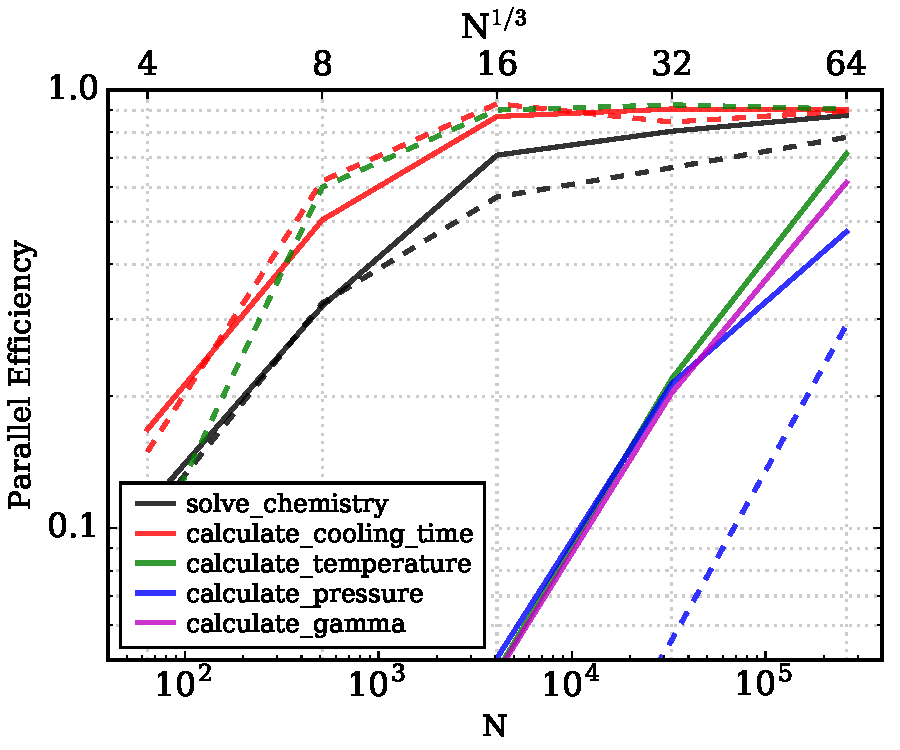
\includegraphics[width=0.98\textwidth]{figures/openmp.pdf}
  \caption{OpenMP parallel efficiency vs. size of fluid container for
    20 threads.  Solid lines show the molecular
    chemistry solver and dashed lines show the tabulated, equilibrium
    model.  For all expensive routines, the efficiency reaches
    $\sim$60\% to 90\% for $16^3$ cells and $\sim$80\% to 90\% for
    $64^3$ cells.}
  \label{fig:openmp}
\end{subfigure}%
\caption{Figures 5 (left) and 6 (right) from
  \citet{2017MNRAS.466.2217S}, showing the single processor
  performance and OpenMP efficiency of \grackle{}'s solvers.}
\label{fig:performance}
\vspace*{-1\baselineskip}
\end{figure}

In addition to the primordial chemistry and cooling, the contribution
to the total cooling rate by metals is calculated by linearly
interpolating over pre-computed tables of heating and cooling rates,
following the method of \citet{2008MNRAS.385.1443S}.
The metal cooling component is calculated within the same subcycle
iteration as the chemistry solver and contributes to the cooling time
time-step limiter.
If using a UV background model, (e.g.,
\citet{2009ApJ...703.1416F} or \citet{2012ApJ...746..125H}),
additional tables also provide photo-ionization, photo-dissociation,
and photo-heating rates for the various atomic and molecular species
in the primordial chemistry as a function of redshift.
The tables distributed with the source code are calculated with the
photo-ionization code, \texttt{Cloudy}, but can in principle be
generated by other similar codes, such as \texttt{Mappings III}
\citep{1993ApJS...88..253S}.

\noindent
{\bf Implementation}
All user-facing \grackle{} functions are written in C due
to the relative simplicity of calling C routines from other
languages, particularly C++ and Fortran.  Most of \grackle{}'s
internal functionality is written in Fortran to make use of the
language's efficient loop and array operations.
The internal machinery is optimized to work with a set of arrays of
densities and internal energies, referred to collectively as a ``fluid
container'', where the arrays can represent either a three-dimensional
grid with inactive ghost zones or a one-dimension set of particles.
The solvers are designed to make the best possible use of cache by
operating on field data in the order in which it is stored in memory.
The core chemistry and cooling computations are performed on
contiguous sub-segments of the field arrays to allow for loops to be
unrolled by compilers for more efficient vector operations.  For
three-dimensional grids, these sub-segments are pencil-beams of all $i$
values for given values $k$ and $j$ in an $i\times j\times k$ cube.
For 1D arrays of particles, analogous divisions can be used to break
the arrays into multiple sub-segments to be passed to the core
functions.

\noindent
{\bf Performance}
In Figure \ref{fig:single-proc}, we
display performance results for \grackle{}'s different solvers.  For
this test, we initialize a 3D fluid container with 64$^{3}$ elements
with density, temperature, and metallicity varying smoothly in each
dimension over the following ranges: $\log (n_{\rm H} /
\textrm{cm}^{-3}) = [-1, 3]$, $\log (T/\textrm{K}) = [1, 8]$, and
$\log (Z/Z_\odot) = [-4, 0]$.  We then evolve the fluid container for
500 years (through repeated called to \texttt{solve\_chemistry}) on a
single core of an Intel Xeon ``Westmere'' E5645 CPU (dual-processor with
6 cores/processor at 2.4 GHz).  On this machine, \grackle{} performs
roughly 0.5-1$\times10^{6}$ full solves per second and at least
10$^{6}$ subcycles per second, depending only slightly on the choice
of solver.  Due to a lack of similar packages, an absolute evaluation
of this performance is difficult.  However, a comparison can be made
to the performance of the \texttt{Enzo} simulation code as a whole.
\citet{2014ApJS..211...19B} perform a weak scaling test of
\texttt{Enzo} on XSEDE's NICS Kraken (a Cray XT4 with quad-core AMD
Opteron CPUs at 2.3 GHz) with a simulation including gravity,
hydrodynamics, and a chemistry solver analogous to \grackle{}'s atomic
solver.  They find that \texttt{Enzo} optimally reaches about 10$^{5}$
full cell updates per second, suggesting that \grackle{} would consume
approximately 20-25\% of the computational cost.

\noindent
{\bf Parallelism}
Because \grackle{}'s functionality requires no communication and is
fully thread-safe once initialized, the library can be easily used
within a simulation code parallelized with a message passing framework
like MPI.  Additionally, all of \grackle{}'s functions are
parallelized with OpenMP by threading the outer loops over which the
solvers are called to operate on the field array sub-segments.  This
allows the library to work within hybrid MPI/OpenMP frameworks, such
as that adopted by the latest version of \texttt{Gadget}.
In Figure \ref{fig:openmp}, we show the OpenMP efficiency of
\grackle{}'s functions for the most and least complex versions
of the solver.  Here, we define parallel efficiency as the ratio of
multi- to single-thread performance.  The test is run using 20 OpenMP
threads on an Intel Xeon E5-2670 v2 CPU (dual-processor with 10
cores/processor at 2.50 GHz) for fluid container sizes from 4$^{3}$ to
64$^{3}$.  For only 16$^{3}$ fluid elements, the efficiency is 60-90\%
for all computationally expensive routines.  The four routines that
show relatively poor efficiency are very inexpensive (for example, see
the 9-species, molecular version of \texttt{calculate\_temperature} as
shown in Figure \ref{fig:single-proc}) and so contribute negligibly to
the total cost.  This parallelism can also be beneficial to pure-MPI codes
where memory requirements force the use of fewer than the total number
of cores on a node, as is often the case.

\subsubsection{\texttt{pygrackle}: The Python Interface}

The Python interface, \texttt{pygrackle}, provides a lower barrier to
entry for accessing \grackle{}'s functionality and thus can be
useful for semi-analytical models \citep[e.g.,][]{2016ApJ...820...71C,
2016MNRAS.459.4209A}, debugging, and education.  The
\texttt{pygrackle} package is distributed with the \grackle{} source
and can be installed once the library has been compiled.  The
additional Python packages on which \texttt{pygrackle} is built
(\texttt{NumPy}, \texttt{Cython}, and \yt{}) are
installable by popular Python package managers, like \texttt{Conda}
and \texttt{pip}.

\texttt{pygrackle} uses an Object-Oriented design centered around
\texttt{FluidContainer} objects.  Analogous to the C \texttt{struct}
by which fields are passed to the \grackle{} library functions, the
\texttt{FluidContainer} object stores field values as \texttt{NumPy}
arrays.  The field arrays use an enhanced version of the
\texttt{NumPy} array, provided by the \yt{} package, that allows
the values to have units that can be expressed and converted
symbolically.  For example, an array, \texttt{x}, of densities in units of
g/cm$^{3}$, can undergo unit conversion by doing:
\texttt{x.to("Msun/kpc**3")}.  The core \grackle{} functions exist as
class methods hanging off the \texttt{FluidContainer} object.  For
example, to calculate the cooling time for a \texttt{FluidContainer}
object, \texttt{fc}, the syntax is
\texttt{fc.calculate\_cooling\_time()}.  The interface layer
connecting the high-level Python data structures to \grackle{}'s C
functions is written in \texttt{Cython}.

\subsection{Community and Usage Metrics}

The first stable version of the \grackle{} library was released in
January 2014.  Since that time, the \grackle{} API has been
implemented in 14 simulation codes and has been used in 23 papers
published in the Astrophysical Journal, Monthly Notices of the Royal
Astronomical Society, and Nature.  The topics of these publications
include galaxy, star, and direct collapse black hole formation; dwarf
and disk galaxies; the high redshift interstellar medium; the
Lyman-alpha forest; history of the Milky Way; reionization; supernova
remnants; metal mixing; and turbulence.  This usage has grown steadily
from year to year, with 1 publication using \grackle{} in 2014, 5 in
2015, 11 in 2016, and 6 within the first two months of 2017.  The
\grackle{} mailing list currently has 68 subscribers, increasing by
roughly 15-20 per year.

Much of \grackle{}'s primordial chemistry solver was first developed
by Peter Anninos and collaborators in the mid-1990s
\citep{1997NewA....2..209A, 1997NewA....2..181A} and incorporated into
the simulation code, \texttt{Enzo} \citep[][licensed under the
  3-clause, revised BSD license]{2014ApJS..211...19B} a few
years later.  As a component of \texttt{Enzo}, the chemistry and
cooling solver was developed through contributions made by many in the
\texttt{Enzo} community, including PI Britton Smith and collaborators
Greg Bryan, Matthew Turk, and Simon Glover.  In response to a call for
a ``common physics package'' to enable a large, multi-simulation
comparison project \citep[AGORA,][]{2014ApJS..210...14K,
  2016ApJ...833..202K}, PI Britton Smith extracted the chemistry and
cooling machinery from \texttt{Enzo} and converted it into a
stand-alone, linkable library that included a number of improvements
and additional features.  The first commit made to the \grackle{}
project was in October 2012.  Since then, the project has progressed
under the same philosophy of feature-driven, community development as
it had as a component of \texttt{Enzo}.  In that time, the code has
received commits from 14 different contributors.

This SSE will establish \grackle{} as a vital software element for the
computational astrophysics community.  It will allow the code to adapt
to the latest technologies that will enable the next generation of
simulations.  It will expand the capabilities of \grackle{} to reach a
larger audience and provide a venue for collaboration and
dissemination of new research.

\section{Development Plan}

The success of the \grackle{} project as a community resource will
ultimately depend on how broadly applicable its functionality is and
its ability to attract new contributions.  The main factors
that will determine whether researchers will choose to make \grackle{}
a destination for new features are 1) the ease with which the source
code can be effectively modified, and 2) whether the code will run
efficiently both now and into, at least, the near future.  Regarding
this second point, efficient use of GPUs and many-core processors are
among the leading concerns of computational astrophysicists.  Tackling
these factors will solidify continued engagement in areas where the
code is now used.  However, breaking into untapped areas of research
will require some supported development in order to reach a minimum
level of usability.  In particular, \grackle{}'s current chemistry
network is not suitable for simulations of present-day star formation,
where additional atomic and molecular species are required.  Expanding
\grackle{}'s functionality to meet the needs of this community is an
explicit goal of this SSE.

The work proposed in this SSE is designed to encourage community
involvement through a series of incremental updates to the underlying
infrastructure followed by the addition of key features that will
enable adoption by additional codes and applications.  Figure
\ref{fig:gantt} displays the timeline for the design and
implementation of each of the milestones comprising this SSE.
\grackle{} is distributed under the 3-clause, revised BSD license and
has no proprietary dependencies.

\begin{figure}
\begin{center}
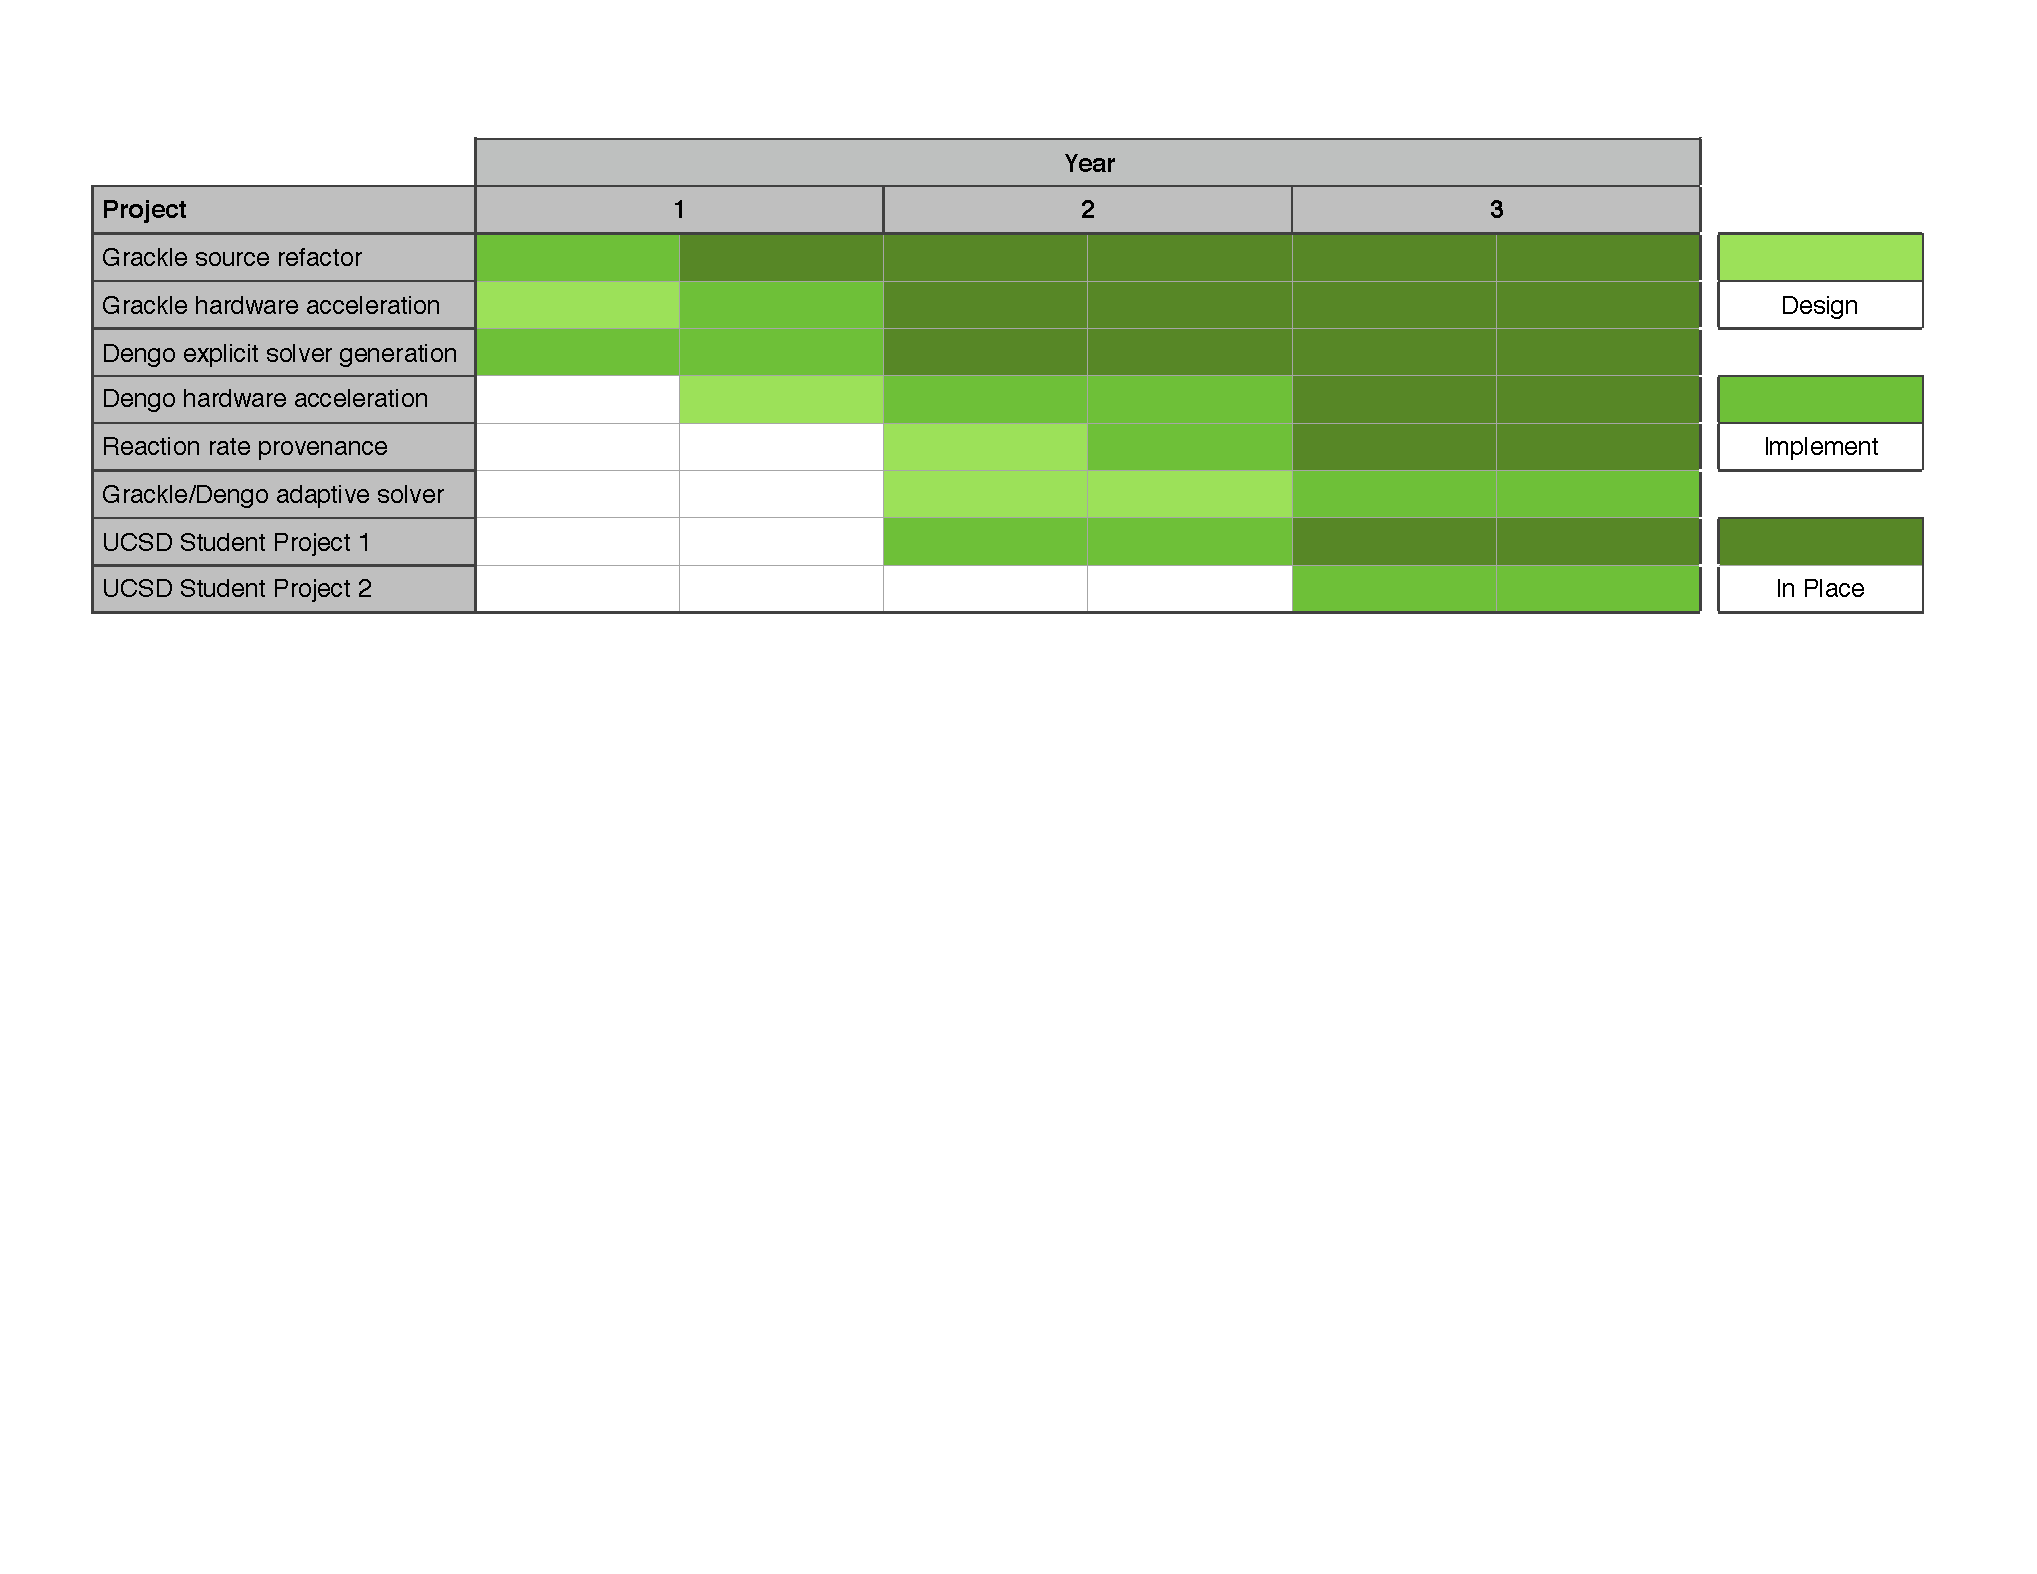
\includegraphics[width=0.7\textwidth]{figures/gantt.pdf}
\caption{Timeline of design and implementation for the three
  development projects in this SSE.}
\label{fig:gantt}
\end{center}
\vspace*{-2\baselineskip}
\end{figure}

\subsection{Year One: Infrastructure Refactor}

The primary goal of the year one development project is to make the
source code substantially more inviting to new contributors and to
build the groundwork for the later projects.  There will be two phases
to this project: 1) expanding the test suite, and 2) porting all
Fortran routines to C.  The planning and commencement of this work
will include direct communication with the \grackle{} user community
via the project's mailing list.  Completion of these phases will be
marked by stable releases.

The design and optimization of the core chemistry and cooling solver
routines in \grackle{} are central factors in making the library fast
enough to be used in extremely large simulations.  However, these
factors also make this the most challenging area of \grackle{} to
work with as a developer.  For example, because there is no simple way
of sharing common/global data or variables between the C and Fortran
routines, the Fortran routines must be handed all parameters, fields,
and rate data as individual arguments.  This results in intimidating
function signatures with dozens of arguments and is only made worse by
the lack of consistency checking between the C and Fortran argument
lists during compilation.  Inconsistencies will result in segmentation
faults whose debugging requires comparison of long lists of function
arguments.  Additional difficulties also include maintaining
consistency in variable type across the C/Fortran interface and the
general confusion that can arise from working in two different
languages at once.  These factors increase the likelihood of bugs and
make the source code significantly less inviting for new
contributors.

The primary advantage of using Fortran for \grackle{}'s most
computationally expensive routines is the speed of array operations.
This is extremely important for \grackle{}, as the code is designed to
work on multiple, large arrays of fields.  This speed advantage was
especially great when the core solvers were originally developed in
the mid-1990s.  However, since that time, advances in the C
programming language, such as the \texttt{restrict} keyword introduced
in the C99 standard \citep{c99}, have made it possible for C code to
be competitive with Fortran.

Phase 1 of the infrastructure refactor will be an expansion of the
test suite to ensure that all functionality and parameter
combinations are covered by answer and unit tests.  The current
test suite adequately covers the most common running modes of the
library, but is insufficient for a full overhaul such as what will
follow.  The completion of phase 1 will be marked by
the release a new stable version of the library.  At the time of
writing, the latest stable release of \grackle{} is version 3.0 with a
3.1 release likely to occur in the next month to cover new features
and bugfixes.  As phase 1 would constitute no change in the library
itself, the resulting release will be a 3.x version (i.e., 3.2 if the
prior version is 3.1).

With a more robust test suite in place, the Fortran code (roughly 7200
lines) can be safely ported to C (phase 2).  The resulting code will
be vastly streamlined as it will no longer be necessary to pass all
required data via function argument.  Instead, the central routines
will be able to access the C \texttt{structs} containing the run-time
parameters, rate data, and field arrays.  In addition, the ease of
calling C routines from Python will allow for the addition of
finer-grained unit tests operating within the existing test suite,
which uses the \texttt{pytest} Python package.  This will also allow
for more of the core functionality to be exposed directly to the user,
as has often been requested.
At present, on startup \grackle{} computes lookup tables from the
functional forms of the reaction rate coefficients.  To enable easier
selection, and greater provenance tracking, we will enable the
\texttt{pygrackle} wrappers to generate pre-computed tables from
functional forms defined in yaml files.  This will provide a method of
experimenting with different rates, such as from different
experimental results or theoretical calculations, while avoiding the
complexity of code generation or full recompilation of the
application.  Finally, with this refactor, the
increased modularity will allow for the implementation of different
solver methodologies.  One potential application of this could be the
fully-implicit solver LSODE \citep{LSODE}.  While LSODE is much slower in many
cases, it allows the individual to specify a more strict convergence
criteria and error threshold than the existing method in \grackle{}.
This may provide utility for situations where \grackle{} struggles
with time-step convergence, such as at extremely high densities.
The result of phase 2 will be a streamlined, more flexible,
refactored source code that will be substantially easier to develop
and will be released as \grackle{} version 4.0.

\subsection{Year Two: Hardware Acceleration}

In order for \grackle{} to continue to be a valuable software element
for the astrophysical community, use of the library must not become
the limiting factor for scaling up simulations.  Because the
calculations performed by \grackle{} are all local to each fluid
element (i.e., solving a given cell does not require information about
neighboring cells), it was straightforward to achieve modest speedup
with OpenMP simply by threading the outer loops for which the core
functions are called.  However, significantly greater speedups can be
achieved by parallelizing the operations within the solvers and taking
advantage of hardware acceleration options currently available on the
latest high performance computing (HPC) systems, such as graphics
processing units (GPUs) and many integrated core architectures (MICs).
For example, \citet{Haidar2016PerformanceAA} report speedups of a
factor of 20-40
for an explicit chemistry network ported to a GPU and even greater
speedups when the GPU is used to compute multiple networks
simultaneously.

National computing facilities used for astrophysical simulations, such
as those in the Extreme Science and Engineering Discovery Environment
(XSEDE) and NCSA Blue Waters, employ acceleration with both GPUs and
MIC architectures.  Implementing separate parallelization strategies,
while potentially resulting in faster code, will likely make the
source code more difficult to work with for new developers.  Instead,
we will develop a new parallelism strategy using the OpenACC standard,
which works with many different architectures.  OpenACC is supported
by PGI, Cray, and GNU compilers.  Similar to OpenMP, OpenACC provides
compiler directives, or pragmas, that allow the programmer to
designate portions of code, particularly loops, to be run on the
accelerator.  Additional directives provide control of when data is
copied to and from the accelerator and also to allow certain data to
exist only in the accelerator's memory.  This strategy is well-suited
to \grackle{}'s core functions which make use of a number of temporary
variables and data to perform many operations on a series of input
arrays.

Adding OpenACC support will happen in year two.  The strategy will be
mapped out in year one during the infrastructure refactor.  We will
make use of local computing resources at the PI's home institution
(San Diego Supercomputer Center, SDSC) for development and testing.
SDSC's Comet supercomputer has 36 NVIDIA dual K80 nodes and 36 NVIDIA
4-way P100 nodes.  SDSC is also an Intel Center of Excellence, hosting
a small Knights Landing (KNL) cluster which will be used for testing
on MIC architectures.
We will also work with system administrators at XSEDE facilities to
provide modules of pre-built \grackle{} libraries to users.  When this
project is completed, we will
release version 5.0 of the \grackle{} library.  Included in this
release will be documentation aimed at new developers with
instructions for parallelizing new features.  To support the broader
impacts of this effort, we will also host a
workshop at UCSD at the end of year two to provide instruction and
a venue for collaboration to researchers interested in contributing
new features.

\subsection{Year Three: Feature Expansion}

The goal of the year three development project is to expand the user
base of \grackle{} to include the present-day star formation
community.  
In contrast to the early Universe, where only H$_{2}$ is important,
star forming clouds in the local Universe are governed by a host of
additional processes, including heat input from cosmic rays and nearby
stars; cooling from molecules like CO, OH, and H$_{2}$O; cooling from
atomic C/O fine-structure emission; and both heating and cooling
effects from dust grains.  Following the detailed chemical structure
of these complex environments is currently outside the range of
\grackle{}'s capabilities.  However, detailed studies of the minimal
chemistry networks required for accurately modeling these systems
\citep{2012MNRAS.421..116G, 2016arXiv161009023G} have paved the way
forward.  Expanding the chemistry solver to include additional species
will help to significantly grow the community of \grackle{} users.
This expansion was also the number one requested feature (by 16 out of
23 total respondents, representing 9 of the supported codes) in a
recent online survey of current \grackle{} users.

In year three, the existing primordial chemistry network will be
expanded to include the network of \citet{2016arXiv161009023G}.  This
is an 18-species network that includes O, O$^{+}$, C, C$^{+}$, CO,
HCO$^{+}$, Si, Si$^{}$+, CH$_{x}$ and OH$_{x}$ (CH$_{x}$ and OH$_{x}$
are pseudo-molecules representing multiple molecules) in addition to
the species currently covered by \grackle{}.
\citet{2016arXiv161009023G} show that this network out-performs all of
the minimal models discussed in \citep{2012MNRAS.421..116G} when
compared to the results of a more sophisticated photo-dissociation
region calculation.  The improvements made in years one and two will
make this effort significantly easier than if it were undertaken
first.  This will also provide a clear path for implementation of
additional networks in the future.  The year three project both adds
functionality and provides a template for user contributions.

This model will be added to \grackle{} using the parallelization
strategy implemented in year two and will be released as a 5.x version
of the \grackle{} library.

\subsection{Engineering and Release Process}

The \grackle{} project follows an established model for development
and releases that is based on other successful community software
projects in which \grackle{}'s developers participate.  The main
source code repository is hosted on
BitBucket.org\footnote{\url{https://bitbucket.org/grackle/grackle}}
and is publicly readable.  Development proceeds via a ``Pull Request''
model that allows for incoming changes to be effectively peer-reviewed
before  being accepted into the main branch.  The \grackle{} library
uses semantic versioning and
is released with numeric versions in an X.Y.Z format, e.g. ``version
2.3.1''.  Changes to the \grackle{} API or a fundamental restructuring
of the source (such as the year one development project) constitute
changes to the X number in a release.  A change in Y occurs when new,
non-API-breaking features are added.  A change in Z marks a release
containing only bugfixes, but no new functionality.

This development process is primarily modelled after that
of the \yt{} community.  The \yt{} project has similar
aims as a cross-platform library for simulations and PI Britton Smith
and Collaborator Matthew Turk have played significant roles in growing
its community and crafting its governance model.  Similar to
\yt{}, the \grackle{} project maintains Community Code of
Conduct and Developer Guide documents to promote a diverse and
inviting community.

\grackle{} is developed using the Mercurial distributed version
control system.  The main repository on BitBucket.org is publicly
readable with write-access currently granted to a handful of the most
experienced developers.  The Pull Request model is used even by those
with write access to the main repo.  In this model, a contributor
``forks'' the main repository, commits changes to their fork, and then
submits a Pull Request allowing other developers to review the
line-by-line changes.  Reviewers leave comments or ``approve'' the
Pull Request and it is eventually accepted or declined in a process
analogous to peer-review for publications.  At the present time, this
usually proceeds with the lead developer (PI Britton Smith) serving as
Pull Request manager by identifying appropriate reviewers (including
himself) and soliciting comments.  As the community continues to grow,
this role can become codified and rotated amongst multiple people.
\grackle{} has received 54 Pull Requests since the first release.

\grackle{} contains a suite of unit and answer
tests that can be run manually using the \texttt{pytest} package.  The
test suite is also run automatically on the central repository and its
forks using the Bitbucket Pipelines continuous integration service.
When a new Pull Request is issued, the results of the test suite are
shown on the Pull Request's web page with links to more detailed
output which can be examined when failures occur.  The test suite
includes a variety of different tests to guard against regression.
Several ``unit tests'' exist to ensure that fundamental
constraints are not violated.  For example, the cooling rates should
match for identical fluid containers that have different internal unit
systems or are in different cosmological reference frames (i.e.,
comoving or proper).  \grackle{} also has a series of ``answer
tests'', wherein the results of specific calculations are compared
against stored values from prior versions.  Finally, to ensure that
the library continues to function as advertised, the test suite
attempts to compile and run the example codes that demonstrate the
APIs.

\grackle{}'s documentation is included in the source and is written in
reStructuredText, which can be converted to HTML and PDF formats
using the Sphinx package.  An HTML rendering of the documentation is
also hosted on
readthedocs.org\footnote{\url{https://grackle.readthedocs.io}},
and is automatically rebuilt when changes are added to the main
repository.

\subsection{Provenance and Reproducibility}

Reproducibility is integral to the scientific process, but can be
difficult to achieve when a calculation relies on a complex software
stack where dependency versions change frequently
\citep{2014arXiv1412.5557J, 2016arXiv161009958L}.  Increased
community involvement in a project, quickening the churn within the
source code, only exacerbates the situation.  In \grackle{}, this
problem is solved by building unique version identifiers directly
into the library.  When the library is compiled, the Mercurial
changeset hash (an effectively unique series of alpha-numeric
characters) is baked into a routine that outputs relevant information
both to a file, called ``GRACKLE\_INFO'', and to the terminal (via
STDOUT) whenever the library's initialize function is called.  In
addition to the changeset hash, the following information is written:
a ``diff'' of any uncommitted changes made to the source, the release
version, all compilation options, and all run-time parameters.
Additionally, \grackle{} maintains a ``CITATION'' file within the
source and in the documentation describing the proper citation
language and BibTex entries to the citable entities.  We will also
follow external examples, where appropriate, to produce machine
readable provenance information \citep[e.g.,][]{force11,
  Fenner097196}.  In these ways, \grackle{} serves as an example to
the community of mechanisms for making reproducibility documents.

\subsection{Alternative Software Packages}

There is a dearth of cross-platform chemistry and cooling packages 
packages available to the astrophysical simulation community.  This
fact was the primary motivator for \grackle{}'s creation.  The main
alternative to \grackle{} is the 
\texttt{KROME}\footnote{\url{http://kromepackage.org/}} package
\citep{2014MNRAS.439.2386G}.  \texttt{KROME} exposes a number of
distinct chemical networks through a Fortran-based API and can also
generate solver code for a custom network defined by the user.
\texttt{KROME} is designed exclusively as a chemistry network solver
and so does not employ cost-saving simplifications, like tabulated
metal cooling and self-shielding models, designed to work in regimes
where direct network solving is computationally prohibitive.
\texttt{KROME}'s solvers are designed to operate on a single fluid
element and do not offer additional parallelization; \texttt{KROME} is
not specifically targeted toward large simulations.

Several other codes exist for solving specific chemistry
networks on single fluid elements, such as 
\texttt{ALCHEMIC} \citep{2010A&A...522A..42S}, \texttt{ASTROCHEM}
\citep{2013MNRAS.431..455K}, \texttt{ASTROCHEM} \citep[][unrelated to
the first \texttt{ASTROCHEM}]{2013A&A...559A..53M}, \texttt{NAHOON}
\citep{2012ApJS..199...21W}, and \texttt{XDELOAD}
\citep{2005Ap&SS.299....1N}.  The \texttt{ASTROCHEM} by
\citet{2013A&A...559A..53M} is the only code hosted in a
publicly-viewable repository.  \texttt{NAHOON} is downloadable as a
static tar file.  \texttt{ALCHEMIC} and \texttt{XDELOAD} are available
upon request.  \texttt{ASTROCHEM} by \citet{2013MNRAS.431..455K} is a
private code.
In addition to the above codes, a number of works have provided tables
of cooling rates \citep{1993ApJS...88..253S, 2009MNRAS.393...99W,
2013MNRAS.434.1043O} that require the surrounding machinery for
interpolating and updating the internal energy to be implemented
independently.
These codes and tables supply important functionality, but it is
not their aim to provide a flexible API to large simulations, nor to
act as a two-way resource that both serves and invites contribution
from the larger community.

The \grackle{} project has focused on providing optimized, easily
adoptable functionality that is independent of simulation code
design.  Through its interoperability with other cross-platform
astrophysical tools like \yt{}, it seeks to exist within the
ecosystem of scientific software rather than alongside it.
Its focus on usability, performance, and community
involvement make it a vital software element to the field of
computational astrophysics.  This focus is underscored by the goals
of the work outlined in this SSE:
to make the source code easier to develop and more inviting to new
contribution; to enhance performance to scale with next-generation
simulations; and to add features that extend the code to new
communities.

\subsection{Advisory Board}

We have formed an advisory board to ensure that the milestones
outlined in this SSE are accomplished satisfactorily and in a timely
fashion.  PI Britton Smith will meet regularly (between 1 and 3 times
per year, via video-conference) with the full board to present updates
on technical progress and progress in achieving the overall goals of
the SSE in terms of growth in users and community involvement.  The
advisory board members are experts in the fields of computational
astrophysics and astrochemistry and have significant experience in the
development (both technical and social) of community software projects
and in parallelizing codes for GPUs and MIC architectures.
{\bf Prof. Greg Bryan} is the original author of the \texttt{Enzo}
simulation code and provides experience with chemistry solving methods
and design of large software projects.
{\bf Dr. Anshu Dubey} was an associate director of the Flash Center
for computational science and one of the lead developers of the
\texttt{FLASH} simulation code \citep{2000ApJS..131..273F,
  2009arXiv0903.4875D}.  Dr. Dubey brings expertise in developing
large adaptive mesh-refinement codes and can advise on adding
\grackle{} support to \texttt{FLASH}.
{\bf Dr. Simon Glover} is a foremost expert in astrochemistry and
chemical networks and has contributed numerous updated chemical rates to
\grackle{}.  Dr. Glover will provide expertise in creating chemical
networks and evaluating their scientific applicability.
{\bf Prof. Michael Norman} is the head of the San Diego Supercomputer
Center and has coordinated development of \texttt{Enzo} and
\texttt{CELLO}/\texttt{Enzo-P}, a peta-scale AMR framework and
simulation code.  Prof. Norman provides experience in software design for
high performance computing and accelerating codes with GPUs and MIC
systems.
{\bf Prof. Stella Offner} is an expert in simulations of present-day
star formation and provides insight into the needs of that community.
Prof. Offner will also advise on adding support for \grackle{} to the
\texttt{ORION} simulation code \citep{2012ApJ...745..139L}.
{\bf Prof. Matthew Turk} is the founder of the \yt{} project and
a core developer of the \texttt{Enzo} simulation code, including
components of the chemistry solver that went into \grackle{}.

The advisory board provides a range of scientific and technical
expertise as well as experience with community software development.
Their input will help to see that milestones are met and that
the project satisfies the needs of the communities it seeks to serve.

\section{Community Growth}\label{sec:community_growth}

Long before it was known by that name, the \grackle{} source code has
been developed as community software as part of the \texttt{Enzo}
code, with significant contributions made by the PI.  The \grackle{}
library was created to fulfill a need
for a cross-platform tool that would enable comparison of the many
different simulation codes in the AGORA project.  PI Smith led the
effort, starting in late 2012, to generalize \texttt{Enzo}'s machinery
and transform it into this tool.  PI Smith also worked with members of
the AGORA project to ascertain what additional functionality would be
required and then made these additions.  Since then, the PI has worked
to grow the \grackle{} community beyond the context of AGORA, and in
that time the number of codes with \grackle{} support grew from the
original 9 in the AGORA project to at least 14.

Strengthening community engagement is critical to the success of the
\grackle{} project after the lifetime of this SSE.  PI Smith has
significant experience organizing scientific software projects as a
core developer of the \texttt{Enzo} code and core developer and
steering committee member of the \yt{} project.  PI Smith authored
\yt{}'s original project governance documentation (YT Enhancement
Proposal 1776) that established the steering committee and codified the
project's procedures for development, team organization, and
acknowledgement of significant contributions.  PI Smith has worked to
model the \grackle{} community after the successes of \yt{} and
\texttt{Enzo}.

The growth of the \grackle{} community will also involve an
educational component in the form of instruction and communication of
new features (such as the new network added in year three) to users,
and training and mentorship for developers, especially after the
significant infrastructure upgrades occuring in years one and two.  PI
Smith has extensive experience in this role, as an instructor at
multiple \texttt{Enzo} and \yt{} users workshops both in the US and
abroad, and in many one-on-one tutorials of \grackle{}, \texttt{Enzo},
and \yt{} with students, at the undergraduate and graduate levels, and
postdocs.  In the summer of 2014 at the Royal Observatory of
Edinburgh, PI Smith organized and taught a series of lectures on
Python skills for scientific computing that was open to all in the
department.  This SSE will provide funding to host a
workshop after year two to provide instruction for new developers in
general best practices and code optimization for hardware
accelerators.  The SSE will also provide funding for team members to
attend conferences and workshops to present on \grackle{} and make
connections to new users.  In these efforts, we will make use of the
lessons and techniques promoted by the Software
Carpentry\footnote{http://www.software-carpentry.org/} project.

This SSE is an investment in the \grackle{} project that will enable
the development projects necessary for making the code a
self-sustaining community resource.  Each component of the work has
been designed to address a critical factor for long term success of
the code: the ease with which it can be developed, its performance
using the latest technologies, and the broadness of its
applicability.

\section{Intellectual Merit}

\grackle{} is a vital scientific software element to the astrophysical
community with demonstrated use in many different simulation codes and
semi-analytic modeling.  The library exposes functionality equally to
simulation codes written in C, C++, Fortran, and Python with an API
that has been designed with careful consideration for maintaining
backward compatibility.  The \texttt{pygrackle} Python interface links
\grackle{} to other cross-platform astrophysical tools like \yt{},
making it a complement to the ecosystem of scientific software.
The \grackle{} project is developed using
best practices and follows an established model for community
development and code releases.  This model includes external review of
source code changes through Pull Requests, automated testing, and
extensive user and developer documentation.

This SSE will enable significant improvements to be made to the
\grackle{} library that will ensure it continues to be a crucial
component of astrophysical research.  The code will be more flexible
and developer-friendly, and will have key features added that will
expand the user base.  The upgraded parallelism will enable
effective utilization of next-generation computing facilities and will
provide a model for developers as they add new features to the code.

\section{Broader Impacts}

This SSE will have a number of important broader impacts that go
beyond its technical achievements.  First, it will provide equal
access to functionality that is necessary for simulation or modelling
research for a wide range of astrophysical topics, including the
formation and evolution of stars, galaxies, black holes, and the
intergalactic medium.
Second, the \texttt{pygrackle} Python module's ease of use lowers the
barrier to entry to using methods that have traditionally only been
available in the context of large, complex simulations.  By
encouraging community contribution, \grackle{} gives researchers
a direct channel to all users of the codes that have adopted the
\grackle{} API, thus providing an avenue for dissemination of
work and for forming collaborations.  These benefits will have the
greatest impact on those with less well-developed professional
networks, who tend to be younger researchers or those from
underrepresented groups.  This SSE will enable the \grackle{} project
to continue to promote a diverse and inclusive community.

By providing this critical functionality equally to simulation codes
that use fundamentally different methods (e.g., Eulerian, Lagrangian,
moving mesh), \grackle{} plays a key role in the comparison of
results, a fundamental pillar of the scientific method.  Evidence of
this is already available in the form of the AGORA simulation
comparison project \citep{2014ApJS..210...14K, 2016ApJ...833..202K},
which has used and continues to use \grackle{} to compare the results
of nine
different simulation codes over a range of galaxy formation problems.

As a well-tested, thoroughly documented library with a well-designed
structure and clear API, \grackle{} also provides an example of the
use best practices for software development and computing.  This is
furthered by the guidance and mentorship that less experienced
developers receive through reviews of Pull Requests and
advice on the mailing list.  These skills can be applied far
beyond computational astrophysics, in other sciences and industry.

\section{Results from Prior Support}

PI Smith has received no prior funding from NSF grants.

\clearpage
\pagenumbering{arabic}
\bibliography{refs}
\end{flushleft}
\end{document}
